% !TEX root = 00_tcc.tex
\clearpage

\section{Conceitos Preliminares}

Segundo~\cite{haykin2009}, no campo de \acrlong{ia} (\acrshort{ia}), uma rede neural é um modelo de
processamento paralelo massivo constituído por uma unidade base, chamada de
nêuron, capaz de armazenar, computar e comunicar informação à seus pares.

Uma \acrshort{ann} é dividida em camadas\footnote{layers} de neurônios onde cada uma conecta a
anterior com a seguinte. Quando formado por várias camadas, é chamado de
aprendizado profundo\footnote{Deep Learning}, em referência à distância entre
camada de \emph{input} e de \emph{output}.

As \acrshort{ann}s possuem várias vantagens em matéria de aprendizado de máquina.
Na forma de aprendizado supervisionado --- apresentadas à dados anteriores ---
são capazes de modelagem preditiva com grande acurácia.  Quando novos dados são
inseridos no modelo, a rede ajusta seus parâmetros se adaptando.
Devido à função de ativação presente no algoritmo, a rede pode mapear relações
não lineares de alta complexidade.

\subsection{Perceptron}

Um Perceptron é a forma mais simples de uma rede neural. É um algoritmo
para classificação binária, usado para distinguir se uma
entrada pertence a um grupo ou não.

O algoritmo consiste em um nêuron com duas características: uma matriz de peso,
representado por $\mathbf{w}$, e um valor de viés, representado por $b$. As
entradas, $x_n$, do modelo são multiplicadas por seus respectivos pesos, somadas entre
si e com o viés. A operação até aqui consiste em uma aplicação linear e pode ser
matematicamente representada como na Equação~\ref{eq:perceptron}.

\begin{equation}
	f(x) = \mathbf{w} \cdot \mathbf{x} + b
	\label{eq:perceptron}
\end{equation}

Em seguida, o resultado é passado para uma função ativadora, no caso do
Perceptron é usado a função degrau\footnote{função de Heavside},
Equação~\ref{eq:heavside}. Essa ativação funciona como separador de positivos e
negativos.

\begin{equation}
	H(x) = \begin{cases}
		1 & x > 0,\\
		0 & \text{caso contrário}
	\end{cases}
	\label{eq:heavside}
\end{equation}

O processo pode ser resumido na Equação~\ref{eq:perceptron2}.  O resultado é o
valor previsto $\hat{y}$, onde 0 e 1 significam cada classe distinta a ser
separada.

\begin{equation}
	\hat{y} = H\left(\sum_{i=1}^{N} w_i \cdot x_i + b\right)
	\label{eq:perceptron2}
\end{equation}

A Figura~\ref{tikz:perceptron} representa visualmente o processo descrito.

% !TEX root = ../00_tcc.tex

\begin{figure}[h]
  \centering

  \scalebox{0.8}{
  \begin{tikzpicture}
    \tikzstyle{neuron}=[circle, draw=black, minimum size = 11mm]
    \tikzstyle{missing}=[draw=none,opacity=0]

	\node[neuron] (out)  at  (4,0)   {$H(\cdot)$};
	\node[neuron] (bias)  at  (4,2)   {$b$};
	\node[]       (resul)  at  (6,0)   {$\hat{y}$};
    \draw[->]     (out)  --  (resul)  ;
    \draw[->]     (bias)  --  (out)  ;

    \foreach \style/\num [count=\i] in {neuron/1,neuron/2,missing/3,neuron/n}{
      \node[\style, draw=none] (input\i)  at  (-1,3-\i*1.5)   {$x_\num$};
	  \node[\style   ]         (nn\i)  at  ( 1,3-\i*1.5)   {$w_\num$};
      \draw[\style,->]         (input\i)  --  (nn\i)  ;
      \draw[\style,->]         (nn\i)  --  (out)  ;
    }

    \node[below of=nn2, node distance=1.5cm] {\LARGE$\vdots$};

  \end{tikzpicture}
}

  \caption{Representação de um Perceptron com $n$ entradas. Fonte: própria.}\label{tikz:perceptron}
\end{figure}


Inicialmente, são atribuídos valores aleatórios aos pesos e ao viés.  É preciso
ajustar os parâmetros de forma que eles mapeiem adequadamente o conjunto entrada
com o saída.  A solução mais usada é aplicar a aproximação numérica
por gradiente descendente.

\subsection{Gradiente Descendente}

O método consiste em alterar os pesos a cada iteração de modo a minimizar uma
função custo pré-definida. A função custo mede o quão distante os pesos
atuais mapearam a entrada do resultado esperado. Comumente é usado o desvio
quadrático médio,
representado na Equação~\ref{eq:rmse},
onde $\hat{y}_{i}$ é o valor previsto e $y_{i}$ é o valor real em uma
i-ésima entrada.

\begin{equation}
	J = \frac{1}{2n} \sum_{i=0}^{n} {(\hat{y}_i - y_i)}^2
	\label{eq:rmse}
\end{equation}

É desejado minimizar o valor de $J$ que, nesse caso, é uma função de
$\mathbf{w}$ e $b$. De forma a simplificar os parâmetros, pode se considerar o
viés como parte de $\mathbf{w}$ e sempre o multiplicar por um. Em notação
matricial fica representado como na Equação~\ref{eq:matriz}.

\begin{equation}
	W^{T} X =
	\begin{bmatrix}
		\theta_0 & \theta_1 & \theta_2 & \cdots & \theta_{n_x}
	\end{bmatrix}
	\begin{bmatrix}
		1 \\ x_1 \\ x_2 \\ \vdots \\ x_{n_x}
	\end{bmatrix}
	\label{eq:matriz}
\end{equation}

Na Equação~\ref{eq:matriz}, $\theta$ são os parâmetros a serem ajustados e
$\theta_0$ é equivalente ao viés.

É sabido que a derivada de uma função é equivalente a inclinação da reta
tangente e quando positiva indica crescimento.  Logo, o problema em questão
precisa diminuir $W$ quando a derivada do custo for positiva e aumentar quando
ela for negativa, pois em ambas situações o custo é minimizado.

A situação é ilustrada na Figura~\ref{tikz:gd}. A linha vermelha
representa o caminho das iterações e a preta as derivadas pontuais.

% !TEX root = ../00_tcc.tex

\begin{figure}[h]
  \centering
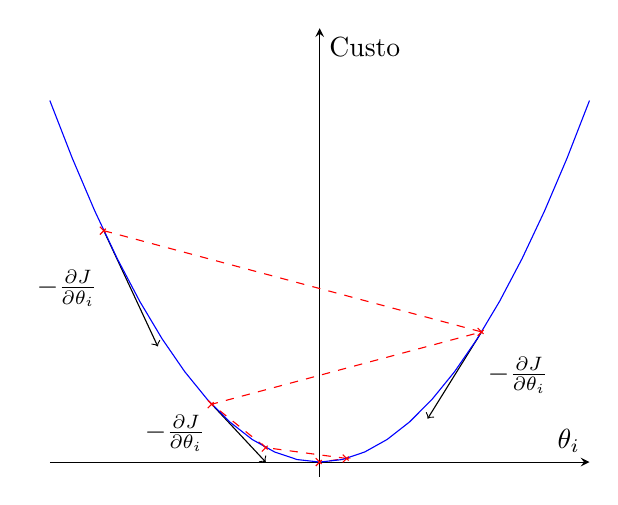
\begin{tikzpicture}
    \begin{axis}[
      clip=false,
      xlabel=$\theta_i$,
      ylabel=Custo,
      xtick={0},
      ytick={0},
      axis y line=center,
      axis x line=middle,
      xmax=5,xmin=-5,
      ymin=-1,ymax=30]

    \addplot[color=red,mark=x,dashed] coordinates {
        (-4,   16)
        (3,     9)
        (-2,    4)
        (-1,    1)
        (0.5,0.25)
        (0,     0)
    };

    \addplot[color=black,->] coordinates {
        (-4,   16)
        (-3,   8)
      } node[pos=0.5, left=0.3cm] {$-\frac{\partial J}{\partial \theta_i}$};

    \addplot[color=black,->] coordinates {
        (3,   9)
        (2,   3)
    }node[pos=0.5, right=0.3cm] {$-\frac{\partial J}{\partial \theta_i}$};

  \addplot[color=black,->] coordinates {
        (-2,   4)
        (-1,   0)
    }node[pos=0.5, left=0.3cm] {$-\frac{\partial J}{\partial \theta_i}$};

    \addplot[blue](x,x*x);

    \end{axis}
\end{tikzpicture}
  \caption{Gradiente descendente em uma função custo quadrática. Fonte: própria.}\label{tikz:gd}
\end{figure}


A Equação~\ref{eq:gd} representa a generalização do cálculo numérico para o
parâmetro $\theta_i$ de uma função custo qualquer. Cada
iteração atualiza a matriz de pesos $W$ de acordo com sua direção de
decrescimento.  O parâmetro $\eta$ é inserido para regular a intensidade da
alteração, chamada taxa de aprendizado\footnote{Learning Rate}.

\begin{equation}
	\theta_{i+1} \leftarrow \theta_i-\eta \frac{\partial J}{\partial \theta_i}(\theta_0, \ldots, \theta_n)
	\label{eq:gd}
\end{equation}

\subsection{Redes Neurais}

Uma rede neural é a generalização do Perceptron para uma quantidade qualquer de
neurônios e uma função ativadora qualquer. Por esse motivo, a rede pode também ser
chamada de Perceptron Multicamada ou \acrshort{mlp}\footnote{\acrlong{mlp}}.

O objetivo da função ativadora no \acrshort{mlp} é introduzir não linearidade no
algoritmo. Caso não fosse aplicada entre os neurônios, a rede seria uma composição
de aplicações lineares, o que é equivalente a uma única aplicação. Funções
ativadoras comuns são a função logística, tangente hiperbólica e a
\acrlong{relu} (\acrshort{relu}).

% !TEX root = ../0_tcc.tex

\begin{figure}[h]
	\centering
	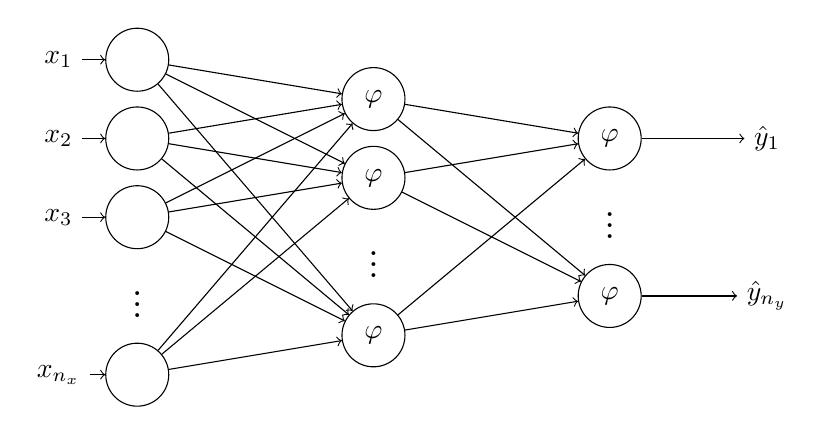
\begin{tikzpicture}
    \tikzstyle{neuron}=[circle, draw=black, minimum size = 8mm]

	\node[] (inp1)  at  (-4,2)   {$x_1$};
	\node[] (inp2)  at  (-4,1)   {$x_2$};
	\node[] (inp3)  at  (-4,0)   {$x_3$};
	\node[] (inp5)  at  (-4,-2)  {$x_{n_x}$};

	\node[neuron] (lay11)  at  (-3,2)   {};
	\node[neuron] (lay12)  at  (-3,1)   {};
	\node[neuron] (lay13)  at  (-3,0)   {};
	\node[]       (lay14)  at  (-3,-1)  {\Large$\vdots$};
	\node[neuron] (lay15)  at  (-3,-2)  {};

	\node[neuron] (lay21)  at  (0,1.5)   {$\varphi$};
	\node[neuron] (lay22)  at  (0,0.5)   {$\varphi$};
	\node[]       (lay23)  at  (0,-0.5)  {\Large$\vdots$};
	\node[neuron] (lay24)  at  (0,-1.5)  {$\varphi$};

	\node[neuron] (out1)    at  (3,1)   {$\varphi$};
	\node[]                 at  (3,0)   {\Large$\vdots$};
	\node[neuron] (out2)    at  (3,-1)  {$\varphi$};

	\node[]       (resul1)  at  (5,1)   {$\hat{y}_1$};
	\node[]       (resul2)  at  (5,-1)  {$\hat{y}_{n_y}$};

	\draw[->]  (out1)  --  (resul1)  ;
	\draw[->]  (out2)  --  (resul2)  ;

	\foreach \i in {1,2,3,5}{
		\draw[->]  (inp\i)  --  (lay1\i)  ;
		\foreach \j in {1,2,4}{
			\draw[->]  (lay1\i)  --  (lay2\j)  ;
		}
	}

	\foreach \i in {1,2,4}{
		\draw[->]  (lay2\i)  --  (out1)  ;
		\draw[->]  (lay2\i)  --  (out2)  ;
	}

	\end{tikzpicture}
	\caption{Representação de uma Rede Neural de 3 camadas, 1 oculta. Fonte: própria.}\label{tikz:nn}
\end{figure}


O processo de treinamento é composto por duas fases, a de \emph{Feedforward} e
a de \emph{\acrlong{bp}} (\acrshort{bp}).  A primeira, é apenas calcular aplicação linear
dos pesos e ativação da entrada até a saída da rede. A segunda consiste em
propagar de forma reversa os gradientes, da saída até a entrada.

Para realizar a \acrshort{bp}, é preciso encontrar a derivada do custo
em relação cada nodo rede. Como cada neurônio é uma aplicação do anterior, a
taxa de variação é calculada através da regra da cadeia, como visto na
Figura~\ref{tikz:bp}.

% !TEX root = ../0_tcc.tex

\begin{figure}[h]
	\centering
	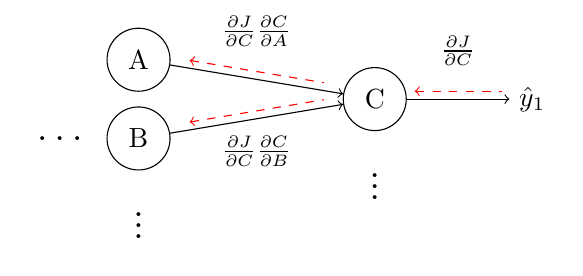
\begin{tikzpicture}
		\tikzstyle{neuron}=[circle, draw=black, minimum size = 8mm]

		\node[]       (lay)  at  (-1,0.5)  {\Large$\dots$};

		\node[neuron] (lay21)  at  (0,1.5)   {A};
		\node[neuron] (lay22)  at  (0,0.5)   {B};
		\node[]       (lay23)  at  (0,-0.5)  {\Large$\vdots$};

		\node[neuron] (out1)    at  (3,1)   {C};
		\node[]                 at  (3,0)   {\Large$\vdots$};

		\draw[->]  (lay21)  --  (out1)  ;
		\draw[->]  (lay22)  --  (out1)  ;
		\node[]       (resul1)  at  (5,1)   {$\hat{y}_1$};
		\draw[->]  (out1)   --  (resul1)  ;


		\begin{scope}[transform canvas={yshift=1mm}]
			\draw[<-, red, shorten >=1mm,  shorten <=1mm,   dashed]  (out1)  --
				(resul1) node[pos=0.5,above=2mm, black] {\small $\frac{\partial J}{\partial C}$};
			\draw[<-, red, shorten >=2.5mm,shorten <=2.5mm, dashed]  (lay21) --
				(out1) (resul1) node[pos=0.5,above=2mm, black] {\small $\frac{\partial J}{\partial C}\frac{\partial C}{\partial A}$};
			\draw[<-, red, shorten >=2.5mm,shorten <=2.5mm, dashed]  (lay22) --
				(out1) (resul1) node[pos=0.5,below=2mm, black] {\small $\frac{\partial J}{\partial C}\frac{\partial C}{\partial B}$};
		\end{scope}

	\end{tikzpicture}
	\caption{\acrshort{bp} através da regra da cadeia. Fonte: própria.}\label{tikz:bp}
\end{figure}


Propagando todas as variações, os pesos da rede são atualizados de acordo com a
Equação~\ref{eq:gd}.

\subsection{Redes Neurais Recorrentes}

Em séries temporais, o valor a ser previsto num determinado tempo $t$ possui
algum grau de dependência com os valores anteriores, não sendo apenas função do
valor $t$. Não é esperado que a irradiação ou a velocidade do vento mudem
bruscamente, mesmo que variações aconteçam.

Uma rede neural comum apenas identifica padrões pelo valor da entrada --- o
instante de tempo nesse caso --- sendo portanto inadequada para situações onde a
proximidade de cada entrada é relevante.

Em tal situação, é preciso implementar uma forma de dependência entre entradas
próximas.  A solução é feita na forma de redes neurais recorrentes. Uma rede
recorrente passa o cálculo de uma predição em $t$ para o próximo cálculo
em $t+1$. A \acrshort{rnn} pode ser representada como na Figura~\ref{tikz:rnn}.

% !TEX root = ../0_tcc.tex

\begin{figure}[h]
	\centering
	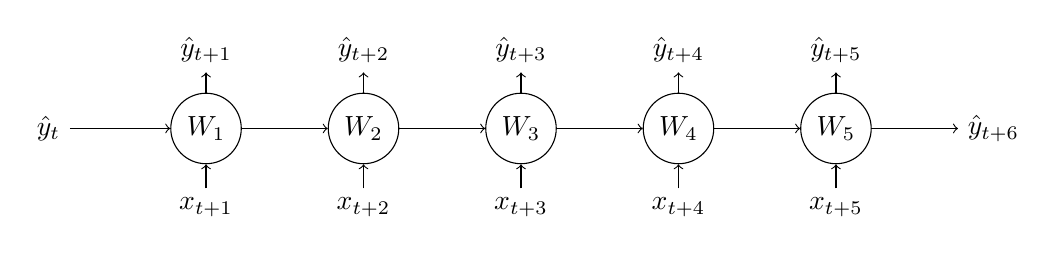
\begin{tikzpicture}
    \tikzstyle{neuron}=[circle, draw=black, minimum size = 8mm]

	\node[]       (n0)  at  (0,0)  {$\hat{y}_t$};
	\node[]       (y)   at  (12,0) {$\hat{y}_{t+6}$};

	\foreach \i in {1,...,5}{
		\node[]       (n\i1)  at  (\i*2,1)  {$\hat{y}_{t+\i}$};
		\node[neuron] (n\i2)  at  (\i*2,0)  {$W_\i$};
		\node[]       (n\i3)  at  (\i*2,-1) {$x_{t+\i}$};

		\draw[->]     (n\i2)  --  (n\i1)  ;
		\draw[->]     (n\i3)  --  (n\i2)  ;
		}

	\draw[->]     (n0)   --  (n12)  ;
	\draw[->]     (n12)  --  (n22)  ;
	\draw[->]     (n22)  --  (n32)  ;
	\draw[->]     (n32)  --  (n42)  ;
	\draw[->]     (n42)  --  (n52)  ;
	\draw[->]     (n52)  --  (y)    ;

	\end{tikzpicture}
	\caption{Representação de uma Rede Neural recorrente. Fonte: própria.}\label{tikz:rnn}
\end{figure}


O gradiente descendente passa a ser aplicado ao longo de \emph{timesteps}
diferentes: \acrshort{bp} através do tempo ou \acrlong{bptt} (\acrshort{bptt}).
Para redes muito profundas, o processo de treinamento com \acrshort{bp} acaba
por gerar um problema chamado de desaparecimento de
gradiente\footnote{vanishing gradient}. Calcular vários gradientes seguidos o
faz tender a 0, visto que o valor entre cada camada possui pequena diferença.
Por isso, treinar tais redes se torna inviável. Alguns modelos propõem soluções
na forma de células que carregam informação entre vários \emph{timesteps} como a
\acrshort{lstm}, desenvolvida por~\cite{hochreiter1997long}.
